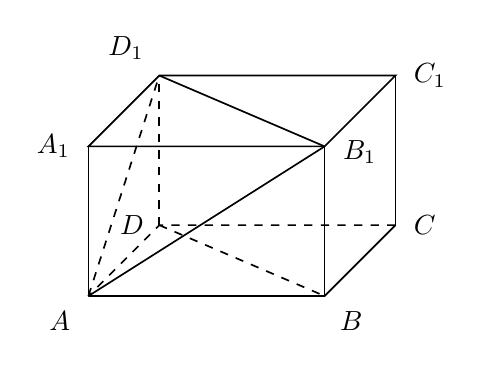
\begin{tikzpicture}[x=1cm,y=1cm,line width=.6pt]
\coordinate (A) at (0,0);
\coordinate (B) at (3,0);
\coordinate (C) at (3.9,0.9);
\coordinate (D) at (0.9,0.9);
\coordinate (A1) at (0,1.9);
\coordinate (B1) at (3,1.9);
\coordinate (C1) at (3.9,2.8);
\coordinate (D1) at (0.9,2.8);
% bottom face
\draw (A)--(B)--(C);
\draw[dashed] (C)--(D)--(A);
\draw[dashed] (D)--(B);
% top face
\draw (A1)--(B1)--(C1)--(D1)--cycle;
\draw (D1)--(B1);
% verticals
\draw (A)--(A1) (B)--(B1) (C)--(C1);
\draw[dashed] (D)--(D1);
% pyramid edges from A
\draw (A)--(B1);
\draw[dashed] (A)--(D1);
\node[below left,xshift=-3pt,yshift=-2pt] at (A) {$A$};
\node[below right,xshift=2pt,yshift=-2pt] at (B) {$B$};
\node[right,xshift=3pt] at (C) {$C$};
\node[left,xshift=-2pt] at (D) {$D$};
\node[left,xshift=-3pt] at (A1) {$A_{1}$};
\node[right,xshift=3pt,yshift=-2pt] at (B1) {$B_{1}$};
\node[right,xshift=3pt] at (C1) {$C_{1}$};
\node[above left,xshift=-2pt,yshift=2pt] at (D1) {$D_{1}$};
\end{tikzpicture}
